%"###############################################
%
% Profils post opératoires
%
%###############################################

% RTUPB
%
%###############################################

\subsubsection{RTUPB}

\begin{figure}[H]
\centering
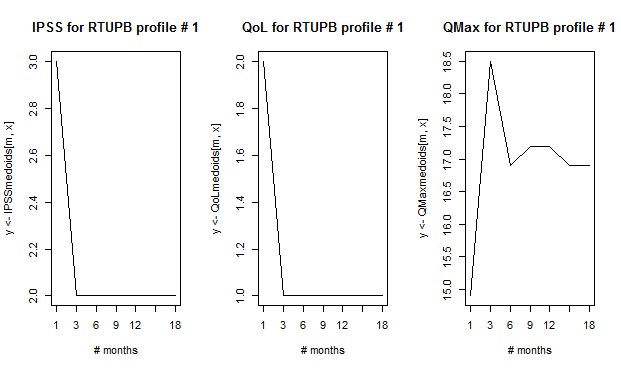
\includegraphics[width=0.75\textwidth]{../Fig/RTUPB/rtupb-profil-post-01.png}
\caption{RTUPB: profil de guérison 1/13}
\label{fig-rtupb-post-profil1}
\end{figure}

Le profil des patients, ci-dessus, montre un bénéfice rapide de l'opération, dès 3 mois, avec une qualité de miction (Qmax) qui progresse spectaculairement à 3 mois, et se stabilise à un régime de croisière à partir de 6 mois (~17.0 ml/s).

\begin{figure}[H]
\centering
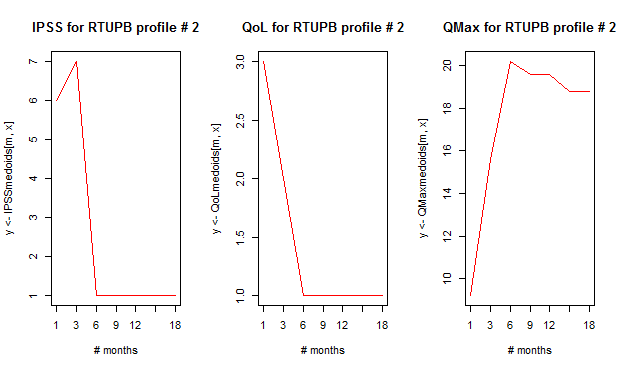
\includegraphics[width=0.75\textwidth]{../Fig/RTUPB/rtupb-profil-post-02.png}
\caption{RTUPB: profil de guérison 2/13}
\label{fig-rtupb-post-profil2}
\end{figure}

Le profil des patients, ci-dessus, montre un bénéfice progressif de l'opération, et stable à partir de 6 mois. La qualité de miction (Qmax) se stabilise à partir de 6 mois entre 18 et 20 ml/s.

\begin{figure}[H]
\centering
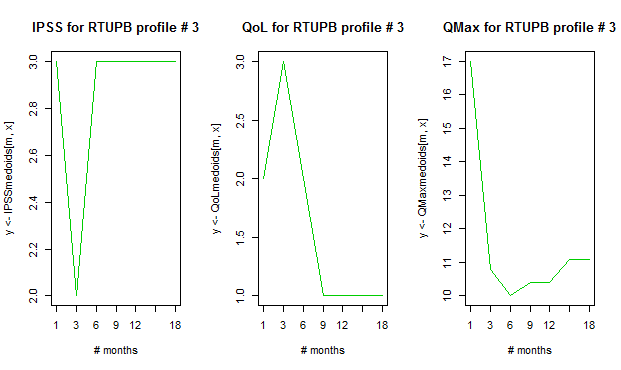
\includegraphics[width=0.75\textwidth]{../Fig/RTUPB/rtupb-profil-post-03.png}
\caption{RTUPB: profil de guérison 3/13}
\label{fig-rtupb-post-profil3}
\end{figure}

Le profil des patients, ci-dessus, montre un ressenti négatif à 3 mois (pic en hausse de QoL, pic en baisse de IPSS), et une dégradation significative de la qualité de miction (Qmax). L'indication QoL par contre redescend à partir de 9 mois. Peut-on interprêter ces résultats comme un résultat décevant de l'opération ?

\begin{figure}[H]
\centering
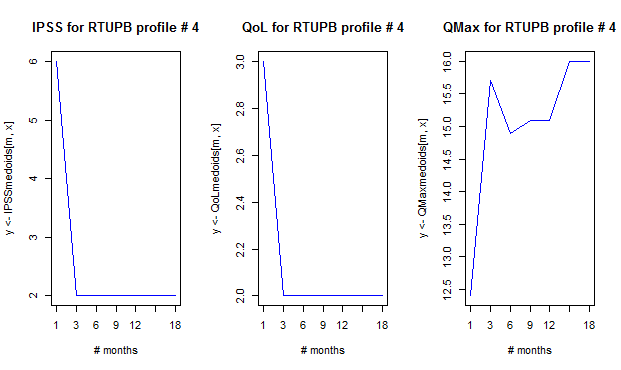
\includegraphics[width=0.75\textwidth]{../Fig/RTUPB/rtupb-profil-post-04.png}
\caption{RTUPB: profil de guérison 4/13}
\label{fig-rtupb-post-profil4}
\end{figure}

Le profil des patients, ci-dessus, est globalement assez proche de celui de la première classe (figure~\ref{fig-rtupb-post-profil1}), avec une évolution différente de la qualité de miction (Qmax) avec des valeurs inférieures tout au long du suivi post-opératoire.

\begin{figure}[H]
\centering
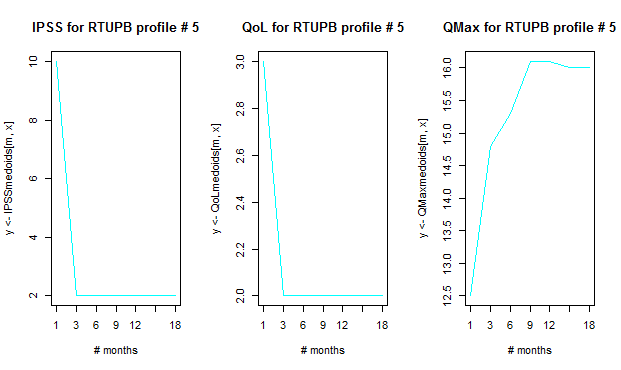
\includegraphics[width=0.75\textwidth]{../Fig/RTUPB/rtupb-profil-post-05.png}
\caption{RTUPB: profil de guérison 5/13}
\label{fig-rtupb-post-profil5}
\end{figure}

Ici aussi, le profil des patients ci-dessus, est assez proche de celui de la première classe (figure~\ref{fig-rtupb-post-profil1}), avec une évolution différente de la qualité de miction (Qmax) plus progressive et sans pic à 3 mois.

\begin{figure}[H]
\centering
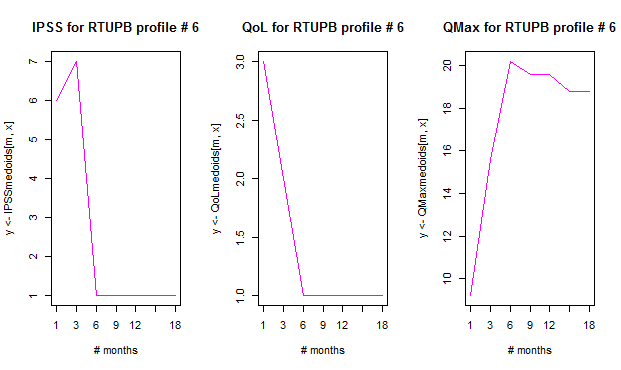
\includegraphics[width=0.75\textwidth]{../Fig/RTUPB/rtupb-profil-post-06.png}
\caption{RTUPB: profil de guérison 6/13}
\label{fig-rtupb-post-profil6}
\end{figure}

Le profil des patients, ci-dessus, est globalement très proche de celui de la deuxième classe (figure~\ref{fig-rtupb-post-profil2}), avec des effets post-opératoires bénéfiques à partir de 6 mois.

\begin{figure}[H]
\centering
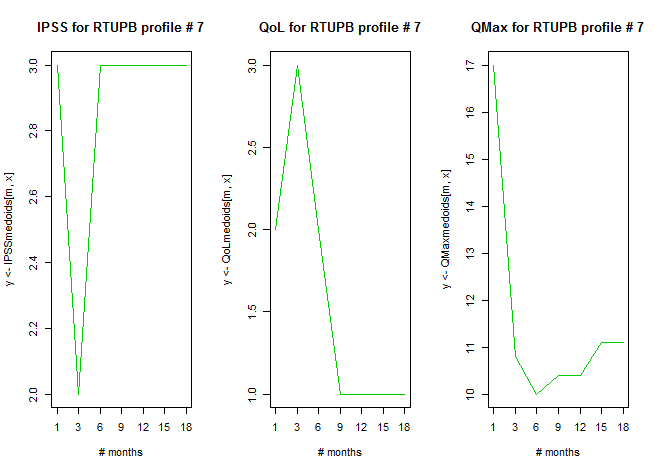
\includegraphics[width=0.75\textwidth]{../Fig/RTUPB/rtupb-profil-post-07.png}
\caption{RTUPB: profil de guérison 7/13}
\label{fig-rtupb-post-profil7}
\end{figure}

Le profil des patients, ci-dessus, est globalement très proche de celui de la troisième classe (figure~\ref{fig-rtupb-post-profil3}), avec des résultats décevants.

\begin{figure}[H]
\centering
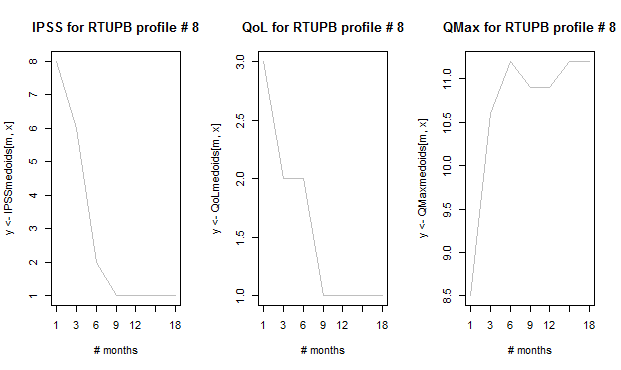
\includegraphics[width=0.75\textwidth]{../Fig/RTUPB/rtupb-profil-post-08.png}
\caption{RTUPB: profil de guérison 8/13}
\label{fig-rtupb-post-profil8}
\end{figure}

Le profil des patients, ci-dessus, montre un bénéfice de l'opération étalé sur les 9 premiers mois. La qualité de miction (Qmax) se stabilise à partir de 6 mois (~11 ml/s).

\begin{figure}[H]
\centering
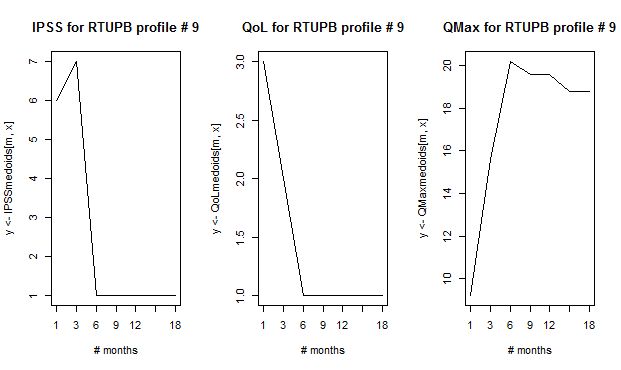
\includegraphics[width=0.75\textwidth]{../Fig/RTUPB/rtupb-profil-post-09.png}
\caption{RTUPB: profil de guérison 9/13}
\label{fig-rtupb-post-profil9}
\end{figure}

Le profil des patients, ci-dessus, est globalement très proche de celui de la deuxième classe (figure~\ref{fig-rtupb-post-profil2}), avec des effets post-opératoires bénéfiques à partir de 6 mois.

\begin{figure}[H]
\centering
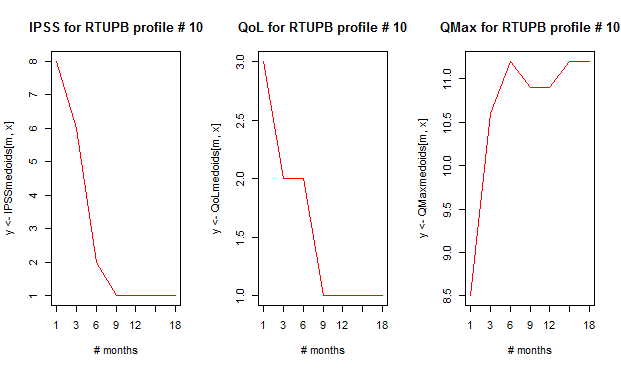
\includegraphics[width=0.75\textwidth]{../Fig/RTUPB/rtupb-profil-post-10.png}
\caption{RTUPB: profil de guérison 10/13}
\label{fig-rtupb-post-profil10}
\end{figure}

Le profil des patients, ci-dessus, très proche de celui de la huitième classe (figure~\ref{fig-rtupb-post-profil8}), montre un bénéfice de l'opération étalé sur les 9 premiers mois. La qualité de miction (Qmax) se stabilise à partir de 6 mois (~11 ml/s).

\begin{figure}[H]
\centering
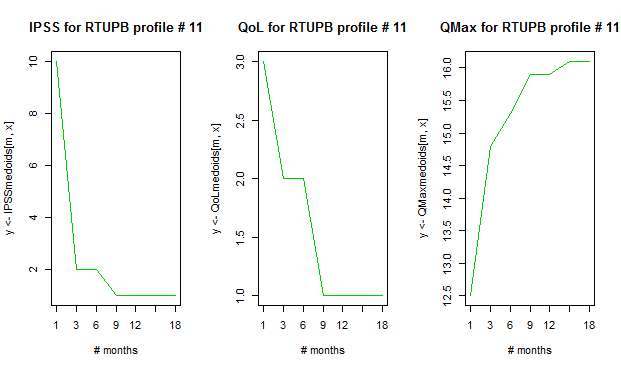
\includegraphics[width=0.75\textwidth]{../Fig/RTUPB/rtupb-profil-post-11.png}
\caption{RTUPB: profil de guérison 11/13}
\label{fig-rtupb-post-profil11}
\end{figure}

Le profil des patients, ci-dessus, assez proche de celui de la huitième classe (figure~\ref{fig-rtupb-post-profil8}), montre un bénéfice de l'opération étalé sur les 9 premiers mois. La qualité de miction (Qmax) est au départ meilleure et se stabilise plus lentement après un an (~11 ml/s).

\begin{figure}[H]
\centering
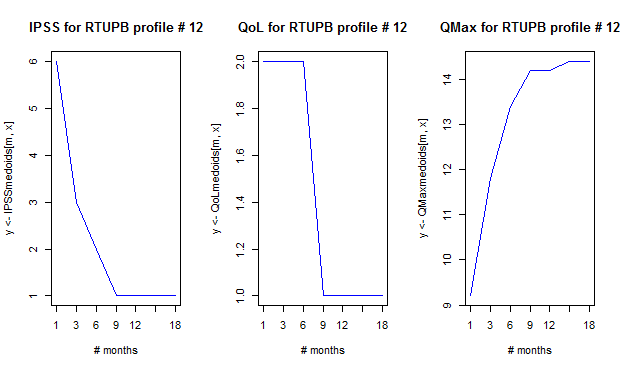
\includegraphics[width=0.75\textwidth]{../Fig/RTUPB/rtupb-profil-post-12.png}
\caption{RTUPB: profil de guérison 12/13}
\label{fig-rtupb-post-profil12}
\end{figure}

Le profil des patients, ci-dessus, assez proche de celui de la huitième classe (figure~\ref{fig-rtupb-post-profil8}), montre un bénéfice de l'opération étalé sur les 9 premiers mois, avec une QoL qui ne descend qu'après 6 mois et une qualité de miction (Qmax) qui se stabilise plus lentement après un an (~14 ml/s).

\begin{figure}[H]
\centering
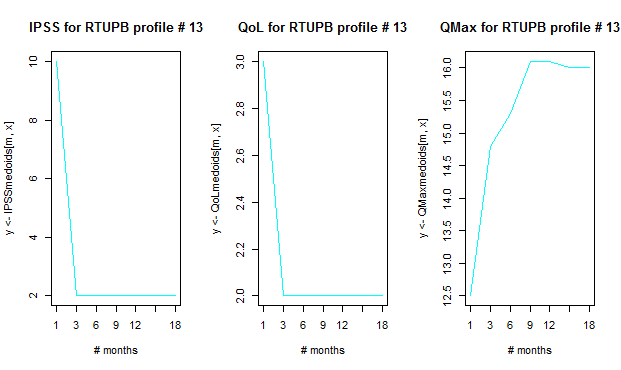
\includegraphics[width=0.75\textwidth]{../Fig/RTUPB/rtupb-profil-post-13.png}
\caption{RTUPB: profil de guérison 13/13}
\label{fig-rtupb-post-profil13}
\end{figure}

Le profil des patients, ci-dessus, est globalement assez proche de celui de la première classe (figure~\ref{fig-rtupb-post-profil1}), avec une évolution différente de la qualité de miction (Qmax) avec des valeurs inférieures tout au long du suivi post-opératoire.

En résumé, il semble donc que d'un point de vue dynamique des profils de guérison, les 13 classes initiales se factorisent en 4 classes:
\begin{itemize}
\item résultat post-opératoire positif à partir de 3 mois (figure~\ref{fig-rtupb-post-profil1}), regroupant 4 des 13 classes initiales,
\item résultat post-opératoire positif à partir de 6 mois (figure~\ref{fig-rtupb-post-profil2}), regroupant 3 des 13 classes initiales,
\item résultat post-opératoire positif à partir de 9 mois (figure~\ref{fig-rtupb-post-profil8}) regroupant 4 des 13 classes initiales,
\item résultat post-opératoire décevant à partir de 3 mois (figure~\ref{fig-rtupb-post-profil3}), regroupant 2 des 13 classes initiales,
\end{itemize}

% VPPBS
%
%###############################################
\subsubsection{VPPBS}

\begin{figure}[H]
\centering
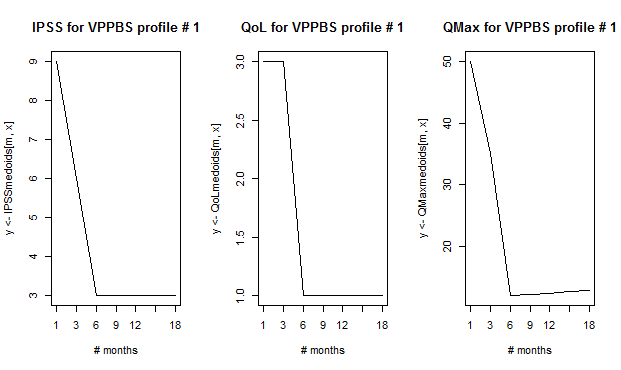
\includegraphics[width=0.75\textwidth]{../Fig/VPPBS/vppbs-profil-post-01.png}
\caption{VPPBS: profil de guérison 1/12}
\label{fig-vppbs-post-profil1}
\end{figure}

Le profil des patients, ci-dessus, montre une amélioration à 6 mois des indicateurs IPSS et QoL, mais en parallèle une dégradation de la qualité de la miction (Qmax). Tous les indicateurs restent ensuite stables au delà des 6 premiers mois.

\begin{figure}[H]
\centering
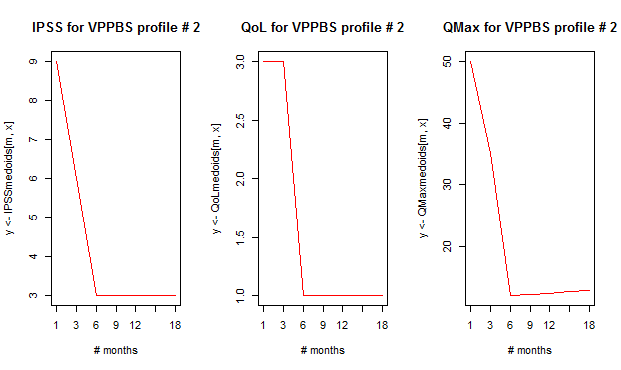
\includegraphics[width=0.75\textwidth]{../Fig/VPPBS/vppbs-profil-post-02.png}
\caption{VPPBS: profil de guérison 2/12}
\label{fig-vppbs-post-profil2}
\end{figure}

Le profil des patients, ci-dessus, est extrêmement très proche de celui de la première classe (figure~\ref{fig-vppbs-post-profil1}.

\begin{figure}[H]
\centering
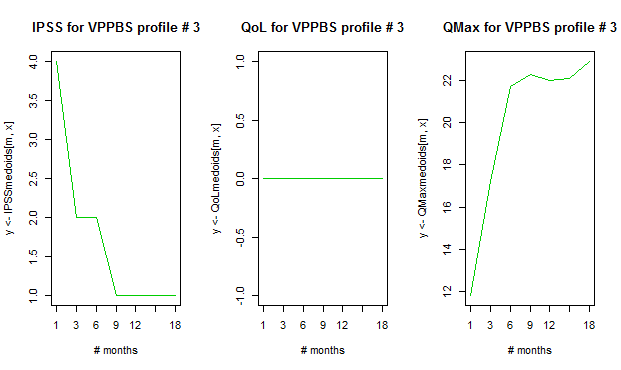
\includegraphics[width=0.75\textwidth]{../Fig/VPPBS/vppbs-profil-post-03.png}
\caption{VPPBS: profil de guérison 3/12}
\label{fig-vppbs-post-profil3}
\end{figure}

Le profil des patients, ci-dessus, montre une amélioration à 9 mois de l'indicateur IPSS (avec un plateau entre 3 et 6 mois), une stagnation de QoL (à 0 initialement, donc pas de souci), et une amélioration de la qualité de la miction (Qmax) très nette sur les 9 premiers mois, plus progressive voire quasi stable ensuite.

\begin{figure}[H]
\centering
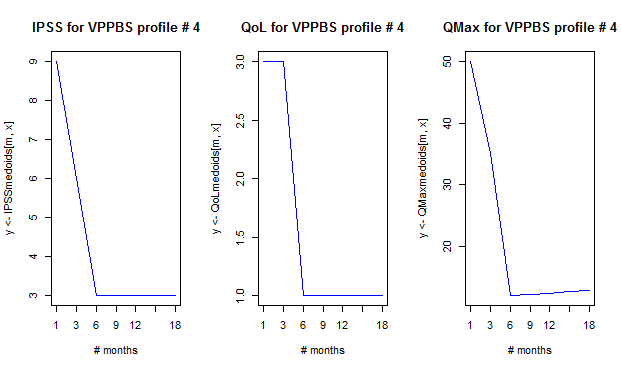
\includegraphics[width=0.75\textwidth]{../Fig/VPPBS/vppbs-profil-post-04.png}
\caption{VPPBS: profil de guérison 4/12}
\label{fig-vppbs-post-profil4}
\end{figure}

Le profil des patients, ci-dessus, est extrêmement très proche de celui de la première classe (figure~\ref{fig-vppbs-post-profil1}.

\begin{figure}[H]
\centering
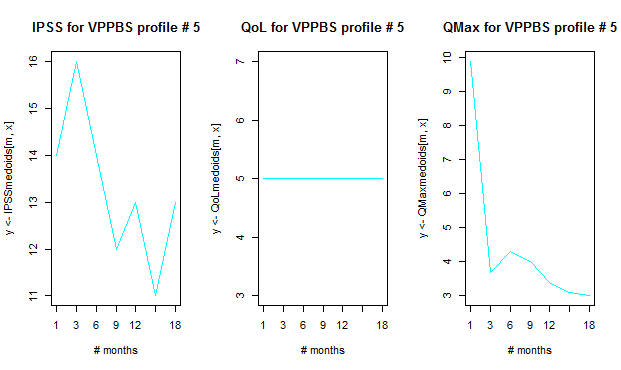
\includegraphics[width=0.75\textwidth]{../Fig/VPPBS/vppbs-profil-post-05.png}
\caption{VPPBS: profil de guérison 5/12}
\label{fig-vppbs-post-profil5}
\end{figure}

Le profil des patients, ci-dessus, montre une amélioration en dents de scie de l'indicateur IPSS (avec 1 pic à 3  mois), une stagnation de QoL à une valeur non nulle, et une dégradation de la qualité de la miction (Qmax) très nette sur les 3 premiers mois, puis plus progressive voire quasi stable ensuite.

\begin{figure}[H]
\centering
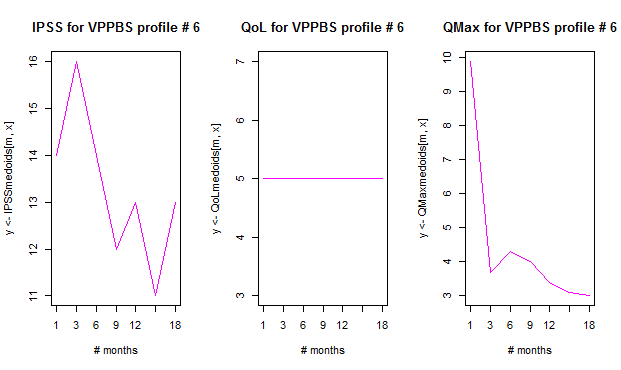
\includegraphics[width=0.75\textwidth]{../Fig/VPPBS/vppbs-profil-post-06.png}
\caption{VPPBS: profil de guérison 6/12}
\label{fig-vppbs-post-profil6}
\end{figure}

Le profil des patients, ci-dessus, est extrêmement très proche du précédent (figure~\ref{fig-vppbs-post-profil5}.

\begin{figure}[H]
\centering
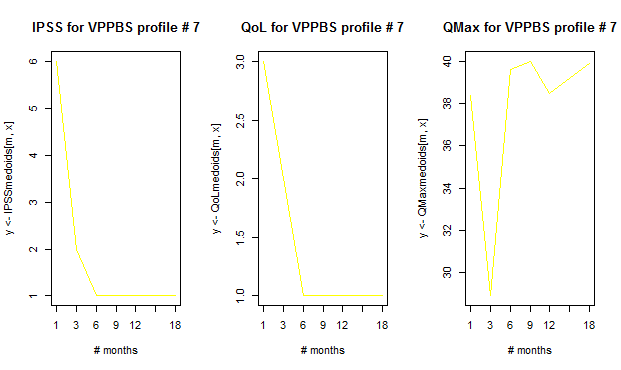
\includegraphics[width=0.75\textwidth]{../Fig/VPPBS/vppbs-profil-post-07.png}
\caption{VPPBS: profil de guérison 7/12}
\label{fig-vppbs-post-profil7}
\end{figure}

Le profil des patients, ci-dessus, montre une amélioration nette des indicateurs IPSS et QoL sur les 6 premiers mois. Ces indicateurs sont ensuite stables. La qualité de la miction (Qmax) s'améliore progressivement à 6 mois et au délà, après une forte chute à 3 mois.

\begin{figure}[H]
\centering
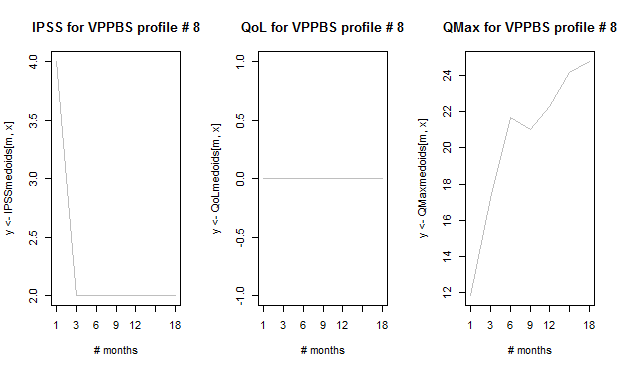
\includegraphics[width=0.75\textwidth]{../Fig/VPPBS/vppbs-profil-post-08.png}
\caption{VPPBS: profil de guérison 8/12}
\label{fig-vppbs-post-profil8}
\end{figure}

Le profil des patients, ci-dessus, est extrêmement assez proche de celui de la troisième classe (figure~\ref{fig-vppbs-post-profil3}, mais nous noterons que la qualité de la miction (Qmax) continue ici à s'améliorer après les 6 premiers mois, jusqu'à la fin du suivi.

\begin{figure}[H]
\centering
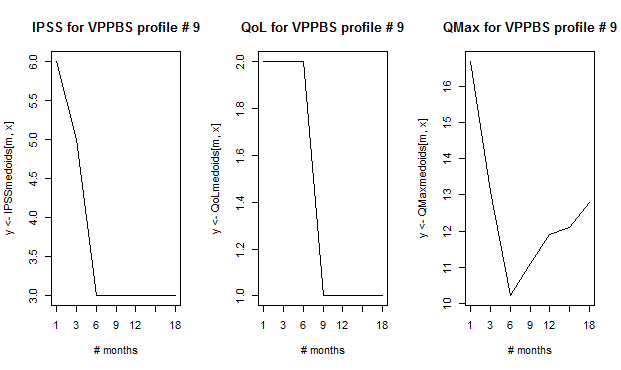
\includegraphics[width=0.75\textwidth]{../Fig/VPPBS/vppbs-profil-post-09.png}
\caption{VPPBS: profil de guérison 9/12}
\label{fig-vppbs-post-profil9}
\end{figure}

Le profil des patients, ci-dessus, est extrêmement très proche de celui de la première classe (figure~\ref{fig-vppbs-post-profil1}.

\begin{figure}[H]
\centering
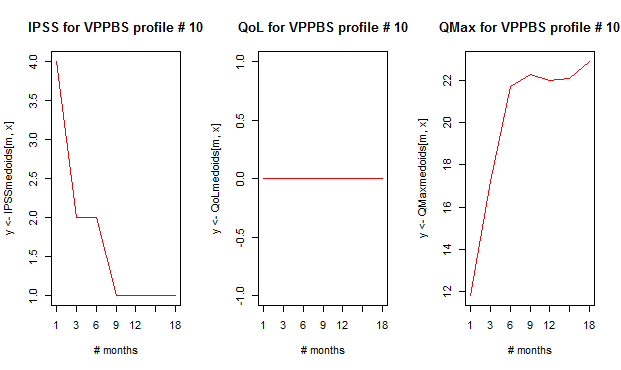
\includegraphics[width=0.75\textwidth]{../Fig/VPPBS/vppbs-profil-post-10.png}
\caption{VPPBS: profil de guérison 10/12}
\label{fig-vppbs-post-profil10}
\end{figure}

Le profil des patients, ci-dessus, est extrêmement assez proche de celui de la troisième classe (figure~\ref{fig-vppbs-post-profil3}.

\begin{figure}[H]
\centering
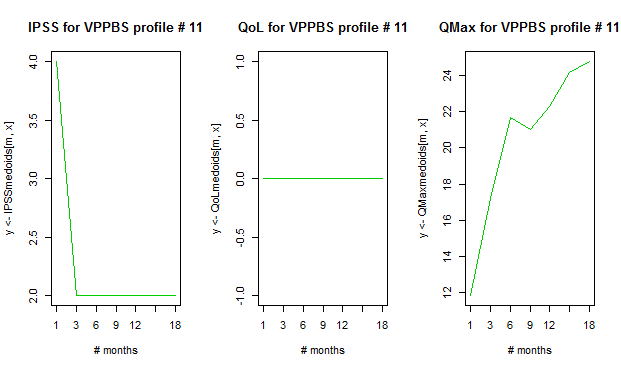
\includegraphics[width=0.75\textwidth]{../Fig/VPPBS/vppbs-profil-post-11.png}
\caption{VPPBS: profil de guérison 11/12}
\label{fig-vppbs-post-profil11}
\end{figure}

Le profil des patients, ci-dessus, est extrêmement très proche de celui de la huitième classe (figure~\ref{fig-vppbs-post-profil8}.


\begin{figure}[H]
\centering
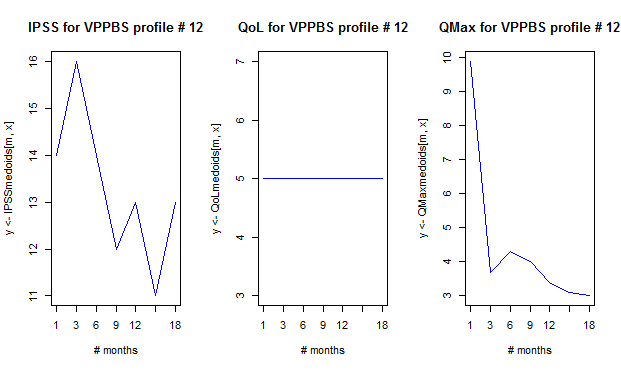
\includegraphics[width=0.75\textwidth]{../Fig/VPPBS/vppbs-profil-post-12.png}
\caption{VPPBS: profil de guérison 12/12}
\label{fig-vppbs-post-profil12}
\end{figure}

Le profil des patients, ci-dessus, est extrêmement très proche de celui de la cinquième classe (figure~\ref{fig-vppbs-post-profil5}.

En résumé, il semble donc que d'un point de vue dynamique des profils de guérison, les 12 classes initiales se factorisent en 5 classes:
\begin{itemize}
\item résultat post-opératoire mitigé: meilleur IPSS/QoL, mais Qmax dégradé (figure~\ref{fig-vppbs-post-profil1}), regroupant 4 des 12 classes initiales,
\item résultat post-opératoire positif dès 3 mois, quasi stable après 9 mois: meilleur IPSS, QoL inchangé, meilleur Qmax (figure~\ref{fig-vppbs-post-profil3}), regroupant 2 des 12 classes initiales,
\item résultat post-opératoire positif dès 3 mois, qui continue à s'améliorer après 9 mois: meilleur IPSS, QoL inchangé, meilleur Qmax (figure~\ref{fig-vppbs-post-profil8}), regroupant 2 des 12 classes initiales,
\item résultat post-opératoire mitigé: amélioration faible et en dents de scie d'IPSS, QoL inchangé, Qmax dégradé à partir de 3 mois (figure~\ref{fig-vppbs-post-profil5}), regroupant 3 des 12 classes initiales,
\item résultat post-opératoire positif à 6 mois, avec une légère amélioration de Qmax après une forte chute à 3 mois (figure~\ref{fig-vppbs-post-profil7}), regroupant 2 des 12 classes initiales,
\end{itemize}

%
%##########################
%# LIENS INTER-PROFILS
%##########################

\subsubsection{Liens entre profils pré et post-opératoires}

\begin{figure}[H]
\centering
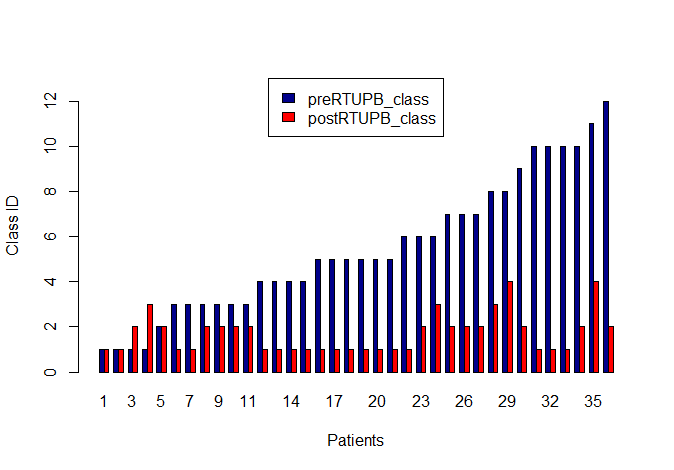
\includegraphics[width=0.75\textwidth]{../Fig/RTUPB/rtupb-histogram-pre-post.png}
\caption{RTUPB: classes pré et post opératoires}
\label{fig-rtupb-histogram}
\end{figure}

\begin{figure}[H]
\centering
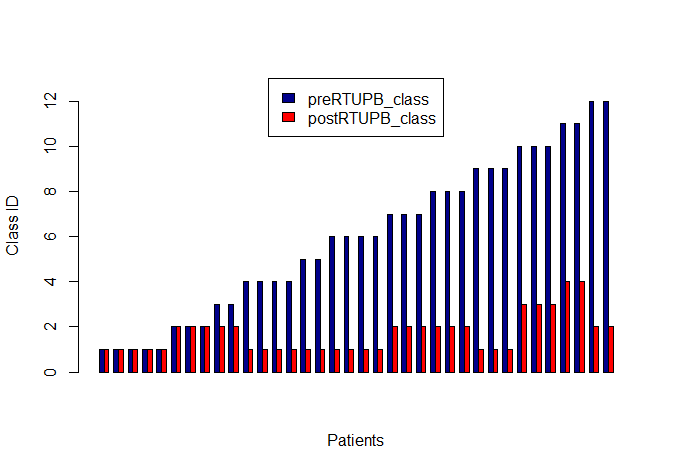
\includegraphics[width=0.75\textwidth]{../Fig/VPPBS/vppbs-histogram-pre-post.png}
\caption{VPPBS: classes pré et post opératoires}
\label{fig-vppbs-histogramFi	}
\end{figure}
